\documentclass[11pt]{article}
\usepackage[margin=1in]{geometry}
\usepackage{amsmath,amssymb,amsthm,booktabs,graphicx}
\usepackage[hidelinks]{hyperref}
\newtheorem{theorem}{Theorem}
\newtheorem{proposition}{Proposition}
\title{Spectral Commutator Telemetry for Two-Level Quantum Control:\\Exact Identities, Pulse Bounds, and Transition-Model Limits}
\author{R. J. Mathews\\Independent Researcher\\\texttt{rjmathews@getqore.ai}}
\date{October 27, 2026 --- v3 technical correction}
\begin{document}
\maketitle
\begin{abstract}
For a two-level Hamiltonian with constant transverse coupling, the operator
commutator diagnostic $\Lambda=\|[H/\hbar,\dot H/\hbar]\|_{op}$ is exactly
one half the coupling times the absolute detuning slope. This identity provides
an interpretable control telemetry channel, but does not by itself determine
transition probability. The Landau--Zener expression gives an exact
relationship for asymptotic linear crossings and a model-dependent surrogate
for finite nonlinear pulses. We retain the archived 90-run simulation
observations, correct the direction and scope of the Fourier-derived
probability inequality, and exhibit a cubic crossing with zero crossing
commutator but nonzero final excited-state population. The defensible result
is a diagnostic identity and a constrained pulse-design heuristic, not a
universal precursor, hardware demonstration, or guaranteed leakage-control law.
\end{abstract}

\paragraph{Revision record.}
The July 2026 v2 corrected the Landau--Zener exponent normalization. This v3
also replaces the spectral \emph{lower} bounds by \emph{upper} bounds on a
clearly labeled slope surrogate, states the Fourier hypotheses, distinguishes
crossing value from peak value, and removes universal pointwise and imminent-
leakage claims. The archived numerical data are unchanged. New scope checks
are post-review tests, not a preregistered extension of the original sweep.
No patent filing is amended by this manuscript revision.

\section{Objects, units, and the exact identity}
In one fixed orthonormal Pauli basis, consider
\begin{equation}
 B(t)=H(t)/\hbar=\tfrac12\bigl(\Delta(t)\sigma_z+\Omega\sigma_x\bigr),
 \qquad \Omega>0\ \hbox{constant},\qquad
 \Lambda(t)=\|[B(t),\dot B(t)]\|_{op}.
 \label{eq:definition}
\end{equation}
The state is a unit vector in $\mathbb C^2$ evolving by
$i\dot\psi=B\psi$. The frequencies $\Delta,\Omega$ have units $s^{-1}$,
and $\Lambda$ has units $s^{-3}$ (radians dimensionless). A time-dependent
basis change requires its connection term and is not covered by simply
conjugating this derivative. The operator norm is not the Frobenius norm.

\begin{proposition}[Constant-coupling identity]
For differentiable detuning,
\begin{equation}
 \Lambda(t)=\tfrac12\Omega|\dot\Delta(t)|. \label{eq:identity}
\end{equation}
\end{proposition}
\begin{proof}
Since $[\sigma_x,\sigma_z]=-2i\sigma_y$,
$[B,\dot B]=-i\Omega\dot\Delta\sigma_y/2$. Use
$\|\sigma_y\|_{op}=1$.
\end{proof}
Thus this scalar is exactly a rescaled slope in the stated model, not an
independent source of predictive information. Nonzero commutator indicates
noncommuting generator change; it neither measures a state's excitation nor
establishes that a transition is imminent. In particular, a constant linear
slope gives constant $\Lambda$ far from as well as at the avoided crossing.

\section{Transition probability: exact model and surrogate}
For $\Delta(t)=\nu t$, constant $\Omega$, and asymptotic ground-state
preparation at $t\to-\infty$, the probability of the excited adiabatic state
at $t\to+\infty$ is the Landau--Zener result~\cite{zener1932}:
\begin{equation}
 P_{LZ}=\exp\!\left[-\frac{\pi\Omega^2}{2|\nu|}\right]
        =\exp\!\left[-\frac{\pi\Omega^3}{4\Lambda}\right].
 \label{eq:lz}
\end{equation}
For a finite nonlinear schedule with crossing $t^*$ and nonzero crossing
slope, define instead
\begin{equation}
 P_{\mathrm{slope}}=
 \exp\!\left[-\frac{\pi\Omega^2}{2|\dot\Delta(t^*)|}\right]
 =\exp\!\left[-\frac{\pi\Omega^3}{4\Lambda(t^*)}\right].
 \label{eq:surrogate}
\end{equation}
This is a surrogate. Its usefulness depends on approximate linearity across
the transition interval, endpoint preparation and separation, and the absence
of additional coherent passages or levels. Nonlinear crossing models have
different transition behavior~\cite{vitanov1999}. A smaller crossing slope
does not establish a universal monotone ordering of arbitrary pulses.
The crossing need not maximize $\Lambda$; a flattened crossing can minimize it.

\paragraph{What ``leakage'' means here.}
The numerical observable is the final excited-adiabatic-state probability
in a two-level system. Identifying it with loss from a computational subspace
requires a separate multilevel encoding and measurement model. This work does
not model decoherence, gate fidelity in a full computational subspace, or
measurement back-action.

\section{Fourier bounds and the corrected inequality}
Use $\hat f(\omega)=\int f(t)e^{-i\omega t}\,dt$ and inverse factor $1/(2\pi)$.
The relevant regularity assumption must be stated for each pulse class.

\begin{theorem}[Spectral moment bound]
Suppose $\Delta$ is represented by its inverse Fourier transform with
$\hat\Delta\in L^1(\mathbb R,(1+|\omega|)d\omega)$. Then for every $t$,
\begin{equation}
 |\dot\Delta(t)|\le\frac{M}{2\pi},\qquad
 \Lambda(t)\le U=\frac{\Omega M}{4\pi},\qquad
 M=\int|\omega|\,|\hat\Delta(\omega)|\,d\omega. \label{eq:fourier}
\end{equation}
\end{theorem}
\begin{proof}
Weighted integrability permits differentiation under Fourier inversion.
Taking the absolute value of
$(2\pi)^{-1}\int i\omega\hat\Delta(\omega)e^{i\omega t}d\omega$
and applying the triangle inequality gives the slope bound; multiply by
$\Omega/2$.
\end{proof}
If $\hat\Delta$ is supported in $[-\omega_c,\omega_c]$, then
$M\le\omega_c\|\hat\Delta\|_1$. For fixed spectral $L^1$ norm, narrowing
bandwidth lowers this \emph{upper bound}; it need not lower the realized
transition probability of an arbitrary schedule.

\paragraph{Derivative formulation.}
For a step-like detuning whose Fourier transform is not an ordinary integrable
function, let $g=\dot\Delta$. If $g$ is continuous and both $g,\hat g$ are
integrable, inversion gives $\Lambda(t)\le\Omega\|\hat g\|_1/(4\pi)$.
Merely assuming $g\in L^1$ does not imply $\hat g\in L^1$.
The infinite linear sweep is outside these integrable-pulse hypotheses.

\paragraph{Probability consequence, with its boundary.}
For $a=\pi\Omega^3/4>0$, $f(x)=e^{-a/x}$ increases on $x>0$.
Consequently, a pulse satisfying the theorem obeys
\begin{equation}
 P_{\mathrm{slope}}\le e^{-a/U}
   =\exp\!\left[-\frac{\pi^2\Omega^2}{M}\right]
   \le\exp\!\left[-\frac{\pi^2\Omega^2}{\omega_c\|\hat\Delta\|_1}\right]
 \label{eq:upper}
\end{equation}
where the last inequality additionally requires the bandlimit and positive
denominators. The zero-denominator case has zero slope and the continuous
surrogate limit zero, not a statement about an actual transition.
Equation~\eqref{eq:upper} bounds the \emph{surrogate only}. Without a separate
bound on $|P_{\mathrm{TDSE}}-P_{\mathrm{slope}}|$, it is neither a rigorous
bound on physical transition probability nor a fundamental leakage floor.
The v2 inequalities and their lower-bound interpretation were incorrect.

\section{Archived simulation evidence}
The retained experiment solves the TDSE with DOP853, relative tolerance
$10^{-11}$ and absolute tolerance $10^{-13}$, starting in the instantaneous
ground state and measuring the final instantaneous excited population.
The 90-run sweep uses three schedules, three couplings $\Omega\in\{0.5,1,2\}$,
and ten crossing slopes. The schedules are linear, tanh, and Gaussian-flattened:
$\dot\Delta=A[1-0.75e^{-t^2/(2\sigma^2)}]$. The latter approaches a slope
four times its crossing value away from the crossing; it does not have its
peak slope at the crossing. The original code fixes the endpoints and widths;
the tanh schedule approaches its declared detuning scale at finite time.

The archived summary reports the following checks. These are a retained
simulation record, not independent experimental validation.
\begin{center}
\begin{tabular}{@{}lr@{}}
\toprule
Quantity & Archived value (rounded)\\
\midrule
Maximum relative identity error, including endpoints & $3.5\times10^{-9}$\\
Maximum final state norm error & $1.6\times10^{-9}$\\
Maximum $|\Delta\ln P|$ in tolerance comparison & $5.8\times10^{-7}$\\
Maximum $|\ln P_{sim}-\ln P_{slope}|$, linear & $0.000574$\\
Same, tanh & $0.002221$\\
Same, Gaussian-flattened & $0.083920$\\
\bottomrule
\end{tabular}
\end{center}
The pooled fitted exponent slope is about $1.003$ against the standard
normalization, rather than the factor-two exponent in the original draft.
This is consistency on those schedules, not proof that $\Lambda(t^*)$ alone
determines every transition. The scaled coupling branches collapse by
nondimensionalization; they are not three independent datasets.

At equal sweep range and total duration, three archived linear versus
Gaussian-flattened comparisons give transition reductions about $8.0$,
$5713.3$, and $349.2$, for $\Omega T$ about $19.1$, $38.2$, and $76.4$.
These particular noiseless comparisons support pulse shaping as a useful
design direction. The slope surrogate is not quantitatively accurate for
all of these strongly flattened pulses and does not prove an exponential
benefit over an arbitrary pulse family or a matched optimal-control baseline.

\begin{figure}[htbp]
\centering
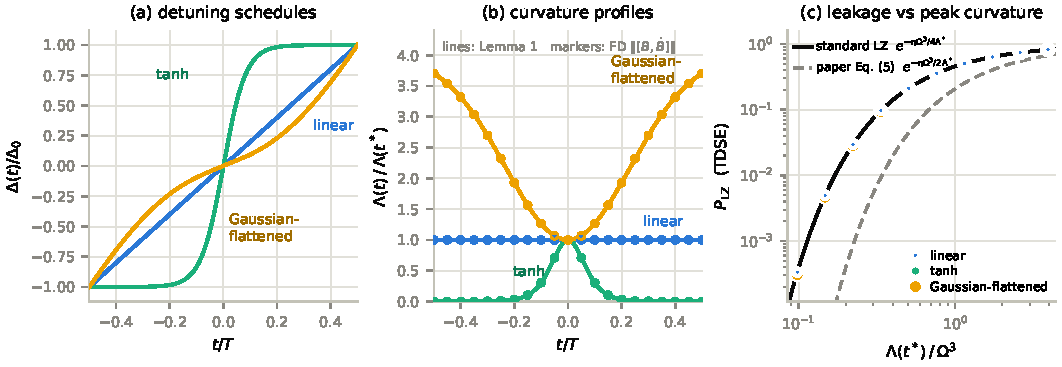
\includegraphics[width=.95\textwidth]{figures/fig_curvature_sweeps.pdf}
\caption{Archived July 2026 sweep visualization, retained unchanged.
The plotted normalization uses the crossing value $\Lambda(t^*)$; any
historical ``peak'' label must be read as crossing value, not the maximum
over time. Agreement of the displayed schedules with the slope model is
approximate, with the residuals reported in the text. The dashed curve is
the superseded factor-two exponent, shown only for comparison.}
\end{figure}

\section{A counterexample to the universal crossing-slope claim}
Set nondimensional $\Omega=1$, $\Delta(t)=t^3$, and
$T_0=30^{1/3}$. Initialize the instantaneous ground state at $-T_0$ and
integrate to $T_0$. The gap minimum is at zero and
$\Lambda(0)=\tfrac12|3t^2|_{t=0}=0$. Nevertheless, a direct TDSE calculation
gives a final excited-state population about
\[
 P_{\mathrm{TDSE}}=0.109231704.
\]
Relative tolerances $10^{-10}$ and $10^{-12}$ agree to better than $10^{-9}$
absolute probability. This example is outside the approximately linear
crossing regime: it invalidates the universal inference from zero crossing
commutator to zero transition, not Eq.~\eqref{eq:identity} or the Fourier
theorem. The finite interval and preparation are part of the example.

\section{Control interpretation and remaining work}
For a declared pulse family, $\Lambda$ can be a slope constraint near the
crossing. Candidate pulses should still be evaluated using the full dynamics
and operational constraints: duration, endpoints, bandwidth, slew rate,
parameter uncertainty, noise and the relevant gate objective. A feedback
implementation additionally needs an estimator and a latency/back-action
model. No such hardware loop is demonstrated here.

For time-varying coupling the algebraic identity becomes
$\Lambda=|\Omega\dot\Delta-\Delta\dot\Omega|/2$ in the same basis, but the
constant-coupling transition relation does not transfer automatically.
Multilevel and multi-qubit systems need their own state, spectral gaps,
transition model and validation. The term ``spectral curvature'' is used as
a diagnostic label, not as an established Riemannian curvature in this paper.

\paragraph{Reproducibility.}
The unchanged sweep data are in \path{results/lzsm_sweeps.json}.
The original harness is \path{sim/lzsm_sweeps.py}.
The post-review executable checks are in \path{tests/test_claim_scope.py}.
The cubic diagnostic is in \path{sim/claim_scope.py}.
Run the following from the repository root:
\begin{verbatim}
python -m unittest discover -s tests -v
python sim/claim_scope.py
\end{verbatim}
These checks do not rerun the entire
90-run archive or establish quantum advantage.

\begin{thebibliography}{9}
\bibitem{zener1932} C. Zener, ``Non-adiabatic crossing of energy levels,''
\emph{Proceedings of the Royal Society A} \textbf{137}, 696--702 (1932).
\bibitem{vitanov1999} N. V. Vitanov and K.-A. Suominen,
``Nonlinear level crossing models,'' \emph{Physical Review A} \textbf{59},
4580--4588 (1999), \url{https://arxiv.org/abs/quant-ph/9811065}.
\bibitem{bracewell2000} R. Bracewell, \emph{The Fourier Transform and Its
Applications}, 3rd ed., McGraw-Hill (2000).
\end{thebibliography}
\end{document}
